\section{Result}\label{result}

Over the week, teams created 1805 entities and 1529 relationships in
total. The number of entities teams created ranged from 24 to 223 (M=82,
SD=39.9), and the number of relationships ranged from 7 to 237 (M=69.5,
SD=51.0). The large variety of modeled data was related to team
strategy, which will be detailed later.

Overview of the survey items indicates that students rated positive on
CAnalytics overall, as shown in Figure~\ref{fig:survey}. CAnalytics were ranked
favorably in all aspects except cognitive load, towards which they had a close
to neutral feeling.

\begin{figure}
\centering
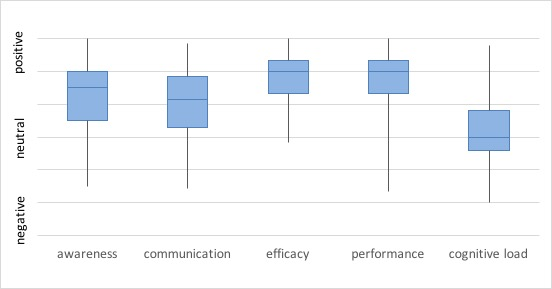
\includegraphics[height=1.5in]{./img/survey_boxchart.jpg}
\caption{Survey responses (box shows Q1-Q3 and median; whiskers show
maximum and minimum)}\label{fig:survey}
\end{figure}

\subsection{Benefits of activity awareness support}\label{benefits-of-activity-awareness-support}

One recurring theme in the subject feedback we collected was that the
collaboration features were helpful for solving the problem on a team basis.
Participants appreciated that the tool added collaboration support to
traditional analytic tools such as Analyst's Notebook, and added analytic
support to common collaboration tools such as Google Doc. One user described
CAnalytics as \emph{``an analysts notebook that multiple people could work on at
once\ldots{}{[}and{]} an analysts version of a Google Doc.''} (P65). Teammates can do individual work while not interfering others. To quote a user's comment:

\emph{``It was much easier to coordinate as a team with CAnalytics because we
could all work on the same system at the same time. Without CAnalytics, we were
forced to do the work separately and compile all the work onto one system after
we had finished.''} (P156)

Students reported being able to see teammate's status made the task more
motivating and enjoyable. The data displayed in the system was not static, but
dynamically updated by teammates, along side with the notifications and other
awareness features each time a collaborator made a change. As participants
commented:

\begin{quote}
During class I wasn't sure if my teammates were doing work for that
class or another thing but then seeing their dot {[}tool indicator{]}
switch between applications on the software and updates pop up on my
screen I knew they were doing work for 231. (P141)
\end{quote}

\begin{quote}
The fact that you can see what other teammates are doing and they can
see what you are doing creates a sense of accountability in terms of
separating the work load. (P51)
\end{quote}

The awareness features were received well. In the survey
(Figure~\ref{fig:survey}) 88\% of the students rated positively on their team
awareness. When asked what features helped them stay aware of team activities,
28 participants mentioned the tool coordinator, 24 mentioned the notification
system, 19 mentioned the history tool, 14 mentioned the real-time update of
user-generated data, 12 mentioned the collaborative editor, and 7 mentioned the
message tool. While the number of mentions does not simply indicate tool
usefulness, it suggests users appropriate these features and were explicitly
aware of their support.

We categorized participants' feedback based on the element of awareness, or
awareness of \emph{what} as emphasized in \autocite{Schmidt2002}, into social
awareness, information awareness, action awareness, history awareness, and
intention awareness, as shown in Table~\ref{tab:awareness}.

% Please add the following required packages to your document preamble:
% \usepackage[table,xcdraw]{xcolor}
% If you use beamer only pass "xcolor=table" option, i.e. \documentclass[xcolor=table]{beamer}
% \usepackage[normalem]{ulem}
% \useunder{\uline}{\ul}{}
\begin{table*}[]
\centering
\small
\label{tab:awareness}
\begin{tabular}{p{3cm}p{10cm}}
\rowcolor[HTML]{9B9B9B}
\multicolumn{1}{c}{\cellcolor[HTML]{9B9B9B}\textbf{Element}}                           & \multicolumn{1}{c}{\cellcolor[HTML]{9B9B9B}\textbf{Example}}                                                                                                                                                                                                                                                                                                                                 \\
\rowcolor[HTML]{C0C0C0}
\begin{tabular}[c]{@{}l@{}} Social awareness\\ \emph{who is present?}\end{tabular}             & CAnalytics helped me stay aware,of my teammates activities because I could see who was logged on in the top,right corner (P123)                                                                                                                                                                                                                                                              \\
\rowcolor[HTML]{EFEFEF}
\begin{tabular}[c]{@{}l@{}}History awareness\\ \emph{Who has done what?}\end{tabular}         & The way you are able to view when and where your teammate made or updated annotations/information was the key to staying aware of what your team has done. It is a great tool in respects to that. For example, I was able to view the changes my team made while I was not using the CAnalytics tool at the same time they were using the history tab. (P171)                               \\
\rowcolor[HTML]{9B9B9B}
\begin{tabular}[c]{@{}l@{}}Information awareness\\ \emph{What is being changed?}\end{tabular} & CAnalyitics was very helpful in keeping us updated on what was being changed/noted/amended by whom and when. This was very beneficial for staying on the same page and knowing what changes were being made so no one individual was out of the loop. (P157)                                                                                                                                 \\
\rowcolor[HTML]{EFEFEF}
\begin{tabular}[c]{@{}l@{}}Action awareness\\ \emph{Who is doing what?}\end{tabular}          & I liked how you could always see what your teammate were viewing on the website. For example I was working on the bluf when my teammates were working on the network part of the program. If I were to come across a piece of information that I thought might be helpful to them I would just tell them. My teammates did the same thing in return. (P51)                                   \\
\rowcolor[HTML]{C0C0C0}
\begin{tabular}[c]{@{}l@{}}Intention awareness\\ \emph{Who is going to do what?}\end{tabular} & CAnalytics showed what tab {[}tool{]} my teammates were working on which helped me be aware of what they were working on. For example, if I saw that one of my teammates was on the network tab, I knew that they were attempting to connect the information that was relevant to one another.,I would then be able to mention any new findings I had that could influence their work (P160)
\end{tabular}
\caption{Subject feedback of awareness instances}
\end{table*}


The positive support of awareness is further corroborated by the interaction
log. For example, we measured the number of entities accessed by collaborators
versus by the author only. While data generated by users is automatically
shared, it is up to collaborators to choose to read the shared information or
ignore information altogether. A high awareness team would keep updated with
collaborators' generated information and read information soon after it is
shared; whereas a low awareness team might experience a significant delay or
even never access it. We found that most teams shared a high proportion of
entities (mean=77.6\%). We found that in average, 77.6\% of the created entities
were accessed by at least one teammate.

One major critique is the lack of sharing support of intermediate analytic
result for close collaboration. When individuals gain an insight from a specific configuration of visualization (e.g.~after a series of zooming, filtering, panning, and highlighting interactions), they did not have a simple channel to communicate that insight together with the
associate views to the team. The team could ``be looking at the same
information but arranged in completely different ways'' (P131). One had to explicitly ask the team to listen to his/her ideas while stopping their own work and turn their to his/her screen. This coordination cost, while seemingly trivial each time, could prohibit one from actively sharing their intermediate findings to withdraw from constant interrupting, which might later lead to team overlooking an important piece of evidence \autocite{Borge2012}.

Another challenge participants faced was the sharing of the frame to model data. Three users mentioned that their team lacked a shared understanding of \emph{what} to annotate. Individuals modeled different levels of details and evidence of various relevance. Four users mentioned that their team did not have a shared understanding of \emph{how} to model data. The teams had inconsistent naming conventions for the same type of evidence. Or they could model the same evidence as different types of entities (e.g. modeling bank as location vs. organization). These misunderstandings can have a big impact on team analysis because such information serves as the foundation for analysis from which a team draws final conclusions.

\subsection{Intertwined data modeling and analysis}\label{Intertwined-data-modeling-and-analysis}

We examined the pattern of data modeling and data analysis by looking at a
visualization of the entire interaction log (e.g.~Figure~\ref{fig:sequence}
shows the interaction log of one team). It was obvious to see teams started with
data modeling since teams at first read documents and made annotations as they
went through. However, teams did not wait to start analysis till they finished
data modeling; instead, the activity of data modeling and data analysis were
highly intertwined. After a certain point, participants frequently switched from
one activity to the other activity . The state transition diagram
(Figure~\ref{fig:transition}) better demonstrates the frequent transitions
between states, in which we encode the number of switches as width of the link.

\begin{figure*}
\centering
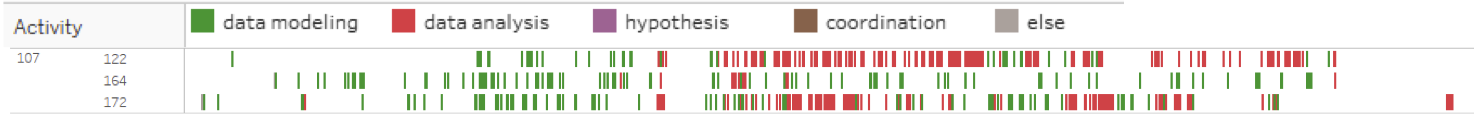
\includegraphics[width=6.5in]{./img/G107-sequence.png}
\caption{Visualization of interaction logs of Team 107. Each row of
colored marks indicates the sequence of top level activities a
participant performed.}\label{fig:sequence}
\end{figure*}

\begin{figure}
\centering
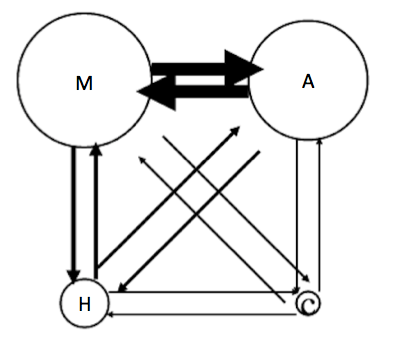
\includegraphics[width=1.5in]{./img/activity_transition-G107.png}
\caption{State transition diagram of interaction logs of Team 107. Each
node is an activity, whose size represents the time spent on the it; a
link represents a switch from one activity to another, whose width
encodes the number of switches.}\label{fig:transition}
\end{figure}

\begin{figure*}
\centering
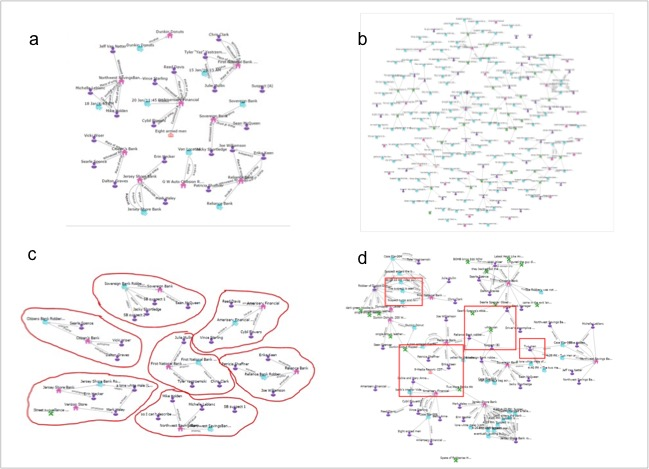
\includegraphics[height=3.5in]{./img/network.jpg}
\caption{User created network graphs. a) Exemplar network with filtering
strategy; b) network with accretion strategy; c) network consisting of
separate clusters; d) network consisting of connected
clusters}\label{fig:network}
\end{figure*}

To look at the consequence of intertwined data modeling and data
analysis, we examined the analytic product teams created, the network
graph in particular because social relationships played the most
critical role in this specific scenario and teams spent most time on
network analysis (as reflected from the log). We found the network views
fell into one of two categories: the networks consisted of 1) separate
clusters, or 2) connected clusters. For example, networks from 8 out of 22 teams
consist of separate clusters (Figure~\ref{fig:network}b). Nodes within a cluster are connected,
representing information space of a robbery case; Nodes between clusters
are nonetheless not connected, indicating each robbery is a
self-contained case. However, these teams still claimed connections
between robberies in their report. Where did they externalize these
connections? Or did the teams simply share orally and held them in mind?
It turns out that these teams documented possible relationships between
robberies in the notepad tool. They used free text to document similarities and common patterns between cases instead of modeled data in the visualization.

In contrast, 6 other teams created networks
composed of connected clusters. While a cluster is still a
representation of a robbery, some of them are connected through an
evidence node. An example is Figure~\ref{fig:network}c, in which we
mark four \emph{connectors} that link the clusters. These connectors
were key evidence that led the teams to hypothesize that those robberies
were related and might be committed by the same criminal group.

While many causes might account for the different network views, we
attempt to interpret the difference from a perspective of uncertainty.
For instance, links within a cluster are factual relationships literally
modeled from raw documents (e.g.~a white van was witnessed at a
location), but links between clusters are often inferences beyond
literally documented (e.g.~a white van at location A is the same van
witnessed at location B). Teams creating separate clusters only
represented facts in the network and held evidence with uncertainty in a
separate artifact. One advantage of distinguishing facts and inferences
is that teams can be aware of assumptions made when making a hypothesis.
And since all inferences are held in one place, teams are forced to
confront them and review their uncertainty iteratively in the process.
However, the strategy also adds difficulty to analysis as analysts may
overlook or fail to combine evidence scattered in different artifacts.

On the contrary, some other teams overlaid facts and inferences in the
same artifact. Both facts and inferences drove the layout of the
network, thus influencing team's framing of the problem. Most teams made
evaluation of the uncertainty of inferences when adding them to the
network. This strategy was relatively more interactive among teammates:
they needed to negotiate, evaluate, and reach consensus on the value and
validity of every inference. To some extent teams might forget whether a
relationship is factual or inferred, and ask whether conclusion derived
from the visualization can be trusted under uncertainty.

From granularity of entities, We noted a distinction between accretion
and filtering strategies in data modeling, similar to findings in a paper prototype study where participants constructed information artifacts on paper \autocite{Carroll2013}. Filtering is selectively modeling of data
and adding to an artifact. Users must decide what information is
relevant, and thus what is to be excluded, as well as what granularity
of information is to model. Filtering requires more team coordination,
because teammates must reach a common ground of the current problem as
well as information needed to answer the problem. Figure~\ref{fig:network}a is an example of filtering, highlighting only
the key information of each robbery and how robberies are connected.

Accretion is an attempt to comprehensively represent the problem by
adding all information to an artifact. Users extract every fact from the
document, regardless of its immediate relevance to the problem.
Accretion costs less coordination as it is relatively mechanical note
taking. A disadvantage of accretion is that it could be time consuming
to model all details and the produced artifact could be fairly complex.
An example is Team 108, who modeled every step the suspects took, which
resulted in many more entities than the average and much more cluttered
network view (Figure~\ref{fig:network}d). Users reported that they
spent too much time in details that they lost the bigger picture:

\begin{quote}
We would find ourselves glued to our computer screens, and spent too
much time on intelligence gathering rather than analysis (P135)
\end{quote}

Different from the result in paper prototype study, however,
participants seemed to be more tempted to accretively add information
with CAnalytics. Students reflected that many annotations did not help
them solve the problem at all because those entities were unrelated to
their problem.

\begin{quote}
I felt that after we were done annotating, we hadn't really accomplished
anything and that we were no closer to solving the case than when we had
started. In the end it didn't really help that we had annotated the
data,
\end{quote}

Why did this happen? We guess both the context of classroom study and
the system design contributed. Unlike in the lab study where teams were
temporarily assembled, teams in a class evaluated peers either
consciously or unconsciously. Such social pressure motivated individuals
to make contributions, and to make \emph{visible} contributions more
than valuable contributions. The awareness features in our system
unfortunately made some contributions more \emph{visible} than others.
For example, creating an annotation would be immediately broadcast to
the team, whereas writing a hypotheses on a notepad produced no
notification, although the text was also shared. The selective awareness
seemed to also exert bias to recognition of contribution.
